\documentclass[11pt,a4paper]{article}

\usepackage[T1]{fontenc}
\usepackage[utf8]{inputenc}
\usepackage[english]{babel}
\usepackage[sc]{mathpazo}
\linespread{1.05}
\usepackage{microtype}
\usepackage[a4paper,margin=2.5cm]{geometry}
\usepackage{amsmath,amssymb}
\usepackage{graphicx}
\usepackage{booktabs,tabularx}
\usepackage{enumitem}
\usepackage[font=small,labelfont=bf,labelsep=colon]{caption}
\usepackage{xcolor}
\usepackage[most]{tcolorbox}
\usepackage[hidelinks]{hyperref}

\definecolor{blueI}{HTML}{2A78D6}
\newtcolorbox{summary}{enhanced, breakable, colback=blueI!5!white, colframe=blueI, boxrule=0pt,
  leftrule=2.4pt, arc=0pt, outer arc=0pt, left=6pt, right=6pt, top=3pt, bottom=3pt}

\title{\textbf{Assessing the group identification}\\[4pt]
  \large What chance means, how real pairs differ from it,\\
  and how the result moves with the parameters}
\author{Matteo Di Sante}
\date{Working note, 23 October 2026\\[2pt]
  \small Companion of the note \emph{Group flights in free flight} (same folder)}

\begin{document}
\maketitle

\begin{summary}
\textbf{The method.} Two pilots are in contact when one of them passes within
$\varepsilon_h=500$~m and $\varepsilon_z=300$~m of where the other was at most
$\delta=2$~min before or after; headings are compared only when both glide
($\theta_{\max}=45^\circ$) and gaps shorter than $g=120$~s are joined. A contact counts
when it lasts at least $\tau^*=38.1$~min. With these values 21.7\% of the paraglider flights and
6.9\% of the hang-glider flights fly in a group at some point, in 17\,169 episodes.

\textbf{Chance.} A pair of the same day is made independent by shifting one flight in time,
by 58~min in the median (Section~\ref{sec:chance}). Its contacts are what route, terrain and
day give without synchrony; $\tau^*$ is the duration at which they are one in ten ($q=0.1$) of
the contacts observed. The length of the shift matters: with only shifts under 30~min
$\tau^*$ would be 53~min, with only shifts over an hour 23~min.

\textbf{Quality.} Real pairs differ from chance in every view: in duration (most short
contacts are chance, few long ones), in delay (5.6 times chance at a few seconds) and in
distance (10 times chance within 100~m at the same instant). The contacts of at least 90~min
have a median delay of 25~s (Section~\ref{sec:views}).

\textbf{Groups.} The median episode lasts 58.2~min and three in four are pairs; the largest
holds 53 flights. Configurations are shorter, 30.4~min in the median
(Section~\ref{sec:structure}).

\textbf{Parameters.} $\delta$ is measured on the delay profile and $\tau^*$ follows from $q$.
The profiles of $\varepsilon_h$, $\varepsilon_z$ and $g$ have no edge, so these three are
definitions; changing them moves the share of time in a group by up to a factor three, mostly
through $\tau^*$ (Section~\ref{sec:tolerances}).

\textbf{Where.} \nolinkurl{/Volumes/SSD_DISANTE/xc-lab/group-identification/}: the chosen run in
\nolinkurl{runs/d120_eh500_ez300_th45_g120_q0.1}, the profiles in \nolinkurl{delays/},
\nolinkurl{separation/} and \nolinkurl{tolerances/}, each with a \texttt{PARAMETERS.md}.
\end{summary}

\tableofcontents

\section{The parameters}

The method of the companion note ran on all the cleaned flights of the FFVL archive,
162\,485 flights of 6\,209 dates; the profiles use a sample of 300 dates. It has three kinds of
parameters (Table~\ref{tab:parameters}).
The \emph{tolerances} say when two positions match: $\delta$, $\varepsilon_h$,
$\varepsilon_z$, $\theta_{\max}$, $g$. The \emph{duration} $\tau^*$ says how long a match must
last to be a contact; it is computed from the share $q$ of chance contacts we accept. The other
\emph{settings} make the computation exact or fast and are fixed by physical bounds.

\begin{table}[h]
\centering
\small
\begin{tabularx}{\textwidth}{@{}l l X@{}}
\toprule
Parameter & Value & How it was set \\
\midrule
$\delta$, largest delay & 2 min & measured on the delay profile, Section~\ref{sec:delay} \\
$q$, accepted false discovery rate & 0.1 & trade-off, Section~\ref{sec:q} \\
$\tau^*$, shortest contact & 38.1 min & computed from $q$ and the null model, Section~\ref{sec:fdr} \\
$\varepsilon_h$, $\varepsilon_z$ & 500 m, 300 m & definitions: profiles without an edge, Section~\ref{sec:tolerances} \\
$g$, longest gap joined & 120 s & definition: gaps of real and chance contacts alike, Section~\ref{sec:tolerances} \\
$\theta_{\max}$ & 45$^\circ$ & no effect on the result, Section~\ref{sec:plateau} \\
$\Delta$, $h_{\max}$, $R_\mathrm{dep}$, $v_{\max}$, $R_s$, $r_{\min}$ & see Section~\ref{sec:fixed} & physical bounds and exactness \\
\bottomrule
\end{tabularx}
\caption{The parameters and how each was set.}
\label{tab:parameters}
\end{table}

\section{What chance means}\label{sec:chance}

\subsection{The null model}

Two pilots who never interact still meet: they take off from the same site, follow the same
ridges and valleys and climb in the same house thermals. The null model of the companion note
builds such pairs from the data. On each date, up to 200 pairs of flights whose takeoffs are
less than $R_s=10$~km apart are drawn; in each, one flight $j$ is replaced by its copy shifted
in time, $\mathbf{x}^s_j(t)=\mathbf{x}_j(t+r)$. The shift is $r=(k^0_j-k^0_i)-\vartheta$, with
$\vartheta$ drawn from the takeoff delays of the pairs of that date, so the copy of $j$ takes off
$\vartheta$ after $i$; only $|r|\ge r_{\min}=2\delta+\Delta=245$~s is accepted. A pair enters
once, with the roles of $i$ and $j$ drawn at random.

\begin{figure}[h]
\centering
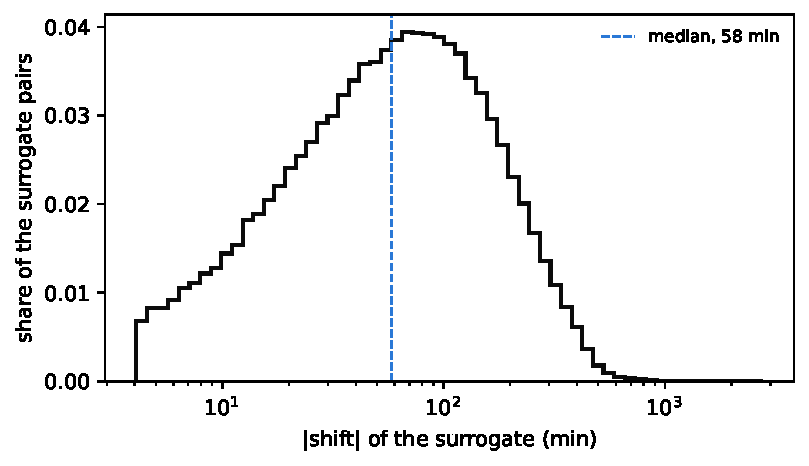
\includegraphics[width=0.62\textwidth]{figures/assessment_shifts.pdf}
\caption{The time shifts $|r|$ of the 248\,741 surrogate pairs of the chosen run, whole
archive.}
\label{fig:shifts}
\end{figure}

What the shifted pair keeps: the route, the terrain, the date, and the takeoff delays of the
day as a distribution. What it destroys: every correspondence within $\delta$, since $|r|>2\delta$.
The shift is far larger than its minimum (Figure~\ref{fig:shifts}): 58~min in the median, and
90\% of the shifts lie between 8~min and 4.4~h. So the copy also flies in the weather of another
hour, with other thermals working and another cloud base.

Chance is therefore an operational notion: the contacts that the same routes give without
synchrony. Two consequences follow.
\begin{itemize}[leftmargin=1.2em]
\item Pilots who use the same thermals at the same time without following each other are in
  synchrony with the weather of the hour, which the shift removes: their contacts count as real.
\item A pilot who follows another deliberately, but more than $\delta$ behind, matches the
  other only beyond $\delta$: the real pair never shows this contact, while a surrogate whose
  shift brings that delay within $\delta$ counts it as chance.
\end{itemize}

\subsection{From the surrogates to the false discovery rate}\label{sec:fdr}

On each date $d$:
\begin{enumerate}[leftmargin=1.6em]
\item $\mathcal{P}_d$ is the set of the pairs $(a,b)$, $a<b$, of flights of the date with
  takeoffs less than $R_s$ apart.
\item The exposure of a pair is the time both fly after departure,
  $h_{ab}=\max\bigl(\min(k^\mathrm{fin}_a,k^\mathrm{fin}_b)-\max(k^\mathrm{dep}_a,k^\mathrm{dep}_b),\,0\bigr)$, and
  $H_d=\sum_{\mathcal{P}_d}h_{ab}$.
\item $\mathcal{S}_d$ is the set of the surrogate pairs $(i,j,r)$; $S_d$ is their exposure, the
  same sum with $j$ shifted:
  $S_d=\sum_{\mathcal{S}_d}\max\bigl(\min(k^\mathrm{fin}_i,k^\mathrm{fin}_j-r)-\max(k^\mathrm{dep}_i,k^\mathrm{dep}_j-r),\,0\bigr)$.
\item $M_d(\tau)$ is the number of contact intervals of the surrogate pairs lasting at least
  $\tau$, and $\rho_{0,d}(\tau)=M_d(\tau)/S_d$ the chance intervals per second of exposure.
\end{enumerate}
Over the archive, with $N(\tau)$ the number of real intervals of the pairs of every
$\mathcal{P}_d$ lasting at least $\tau$:
\begin{equation}\label{eq:fdr}
  C(\tau)=\sum_d \rho_{0,d}(\tau)\,H_d,\qquad
  \widehat{\mathrm{FDR}}(\tau)=\frac{C(\tau)}{N(\tau)},\qquad
  \tau^*=\min\bigl\{\tau:\ \widehat{\mathrm{FDR}}(\tau)\le q\bigr\}.
\end{equation}
$C(\tau)$ is the number of intervals lasting at least $\tau$ that chance alone would give the
real pairs. It is summed date by date because the surrogates are a sample of the pairs of each
date; dates without surrogates add to $N$ only. $\tau$ runs over the grid $\{0,5,\dots,14\,400\}$~s.

\subsection{How much the shift matters}\label{sec:shift-classes}

The false discovery rate was recomputed with only the surrogate pairs of each date whose shift
falls in one class, each class with its own exposure $S_d$ and intervals. The classes are
compared on the 2\,737 dates (of 6\,209) that have surrogates in each of them
(Table~\ref{tab:shift-classes}).

\begin{table}[h]
\centering
\small
\begin{tabular}{@{}l r c c c c@{}}
\toprule
Surrogates & pairs & $\widehat{\mathrm{FDR}}$(10 min) & $\widehat{\mathrm{FDR}}$(30 min) & $\tau^*$ (min) & 5--95\% over dates \\
\midrule
all shifts & 241\,824 & 0.48 & 0.16 & 38.2 & 37.0--41.5 \\
$|r|<30$ min & 69\,444 & 0.73 & 0.31 & 53.3 & 49.7--72.0 \\
$|r|\ge60$ min & 119\,687 & 0.26 & 0.05 & 23.0 & 21.1--24.4 \\
\bottomrule
\end{tabular}
\caption{The false discovery rate and $\tau^*$ ($q=0.1$, $\delta=2$~min) with the surrogates of
one class of shifts, on the 2\,737 dates with surrogates in each class.}
\label{tab:shift-classes}
\end{table}

Short shifts give 2.8 times the chance of long ones at 10~min and 5.7 times at 30~min, and
$\tau^*$ goes from 23~min with
shifts of an hour or more to 53~min with shifts under 30~min; with all the shifts it is 38~min,
as on the whole archive. Short shifts keep the weather of the hour, but they also bring within
$\delta$ the pilots who follow each other a few minutes apart, and the delay profile shows that
these are many: real correspondences are still 2 to 3 times chance between 195 and 500~s
(Section~\ref{sec:delay}). The two effects cannot be separated here. The length of the shift
decides what counts as chance and moves $\tau^*$ by more than a factor two; we keep the shifts that
follow the takeoff delays of the day.

\section{Real pairs against chance}\label{sec:views}

Three views compare the real pairs with their surrogates: how long their contacts last, at
which delay the two pilots match, and how far apart they are at the same instant.

\subsection{Duration}

\begin{figure}[h]
\centering
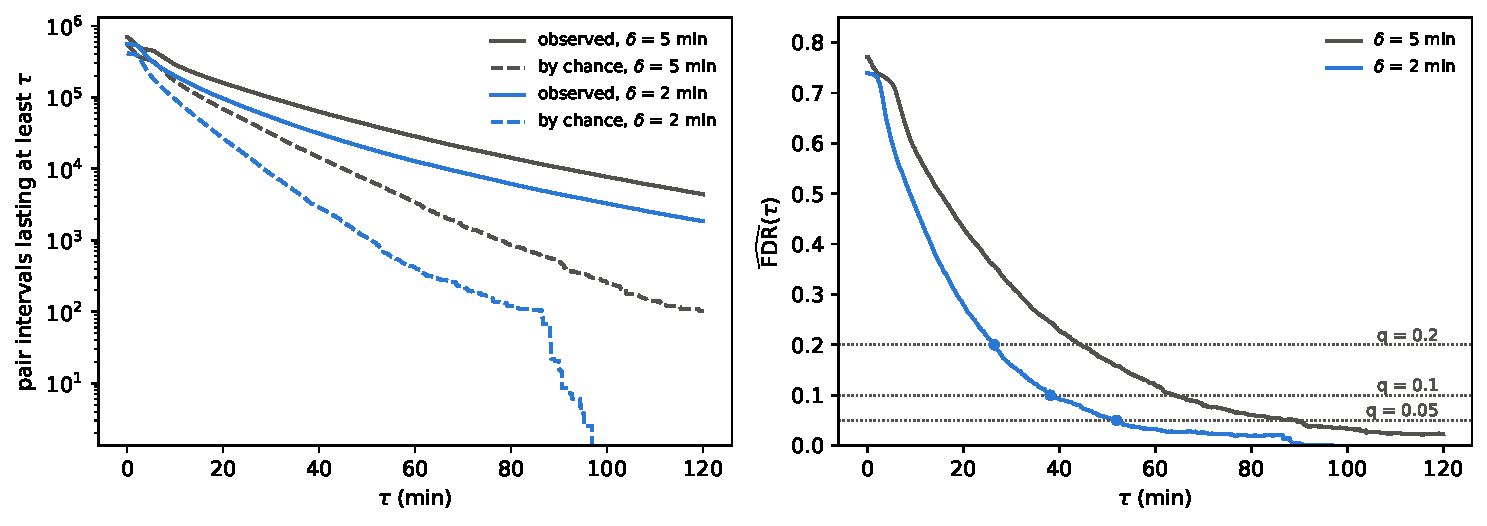
\includegraphics[width=\textwidth]{figures/assessment_fdr.pdf}
\caption{Left: real pair intervals lasting at least $\tau$ (solid) and those chance alone
gives (dashed), with $\delta=5$~min (grey) and $\delta=2$~min (blue), on the whole archive.
Right: their ratio, the false discovery rate of Eq.~\eqref{eq:fdr}; dots mark $\tau^*$ for
$q=0.05$, 0.1 and 0.2 with $\delta=2$~min.}
\label{fig:fdr}
\end{figure}

Most contacts are chance (Figure~\ref{fig:fdr}): 74\% of all pair intervals with
$\delta=2$~min (77\% with 5~min), 47\% of those lasting 10~min, 16\% of those lasting 30~min.
Short contacts therefore say little; only long ones are mostly real. This is why $\tau^*$ is
tens of minutes: it is the duration at which the real contacts outnumber chance by the factor
$1/q$. Resampling the dates 200 times moves $\tau^*$ by a few minutes (Table~\ref{tab:q}), so
the curve, and not the noise of the surrogates, sets it.

\subsection{Delay}\label{sec:delay}

For every delay $l$, the correspondences $(t,t+l)$ of the real pairs and of the surrogate pairs
were counted, per second of exposure, with a window of 15~min on 300 random dates
(58\,910~h of real exposure):
\begin{equation}\label{eq:profile}
  R(l)=\frac{\text{real correspondences at delay } l \text{ per second of exposure}}
             {\text{chance correspondences at delay } l \text{ per second of exposure}} .
\end{equation}

\begin{figure}[h]
\centering
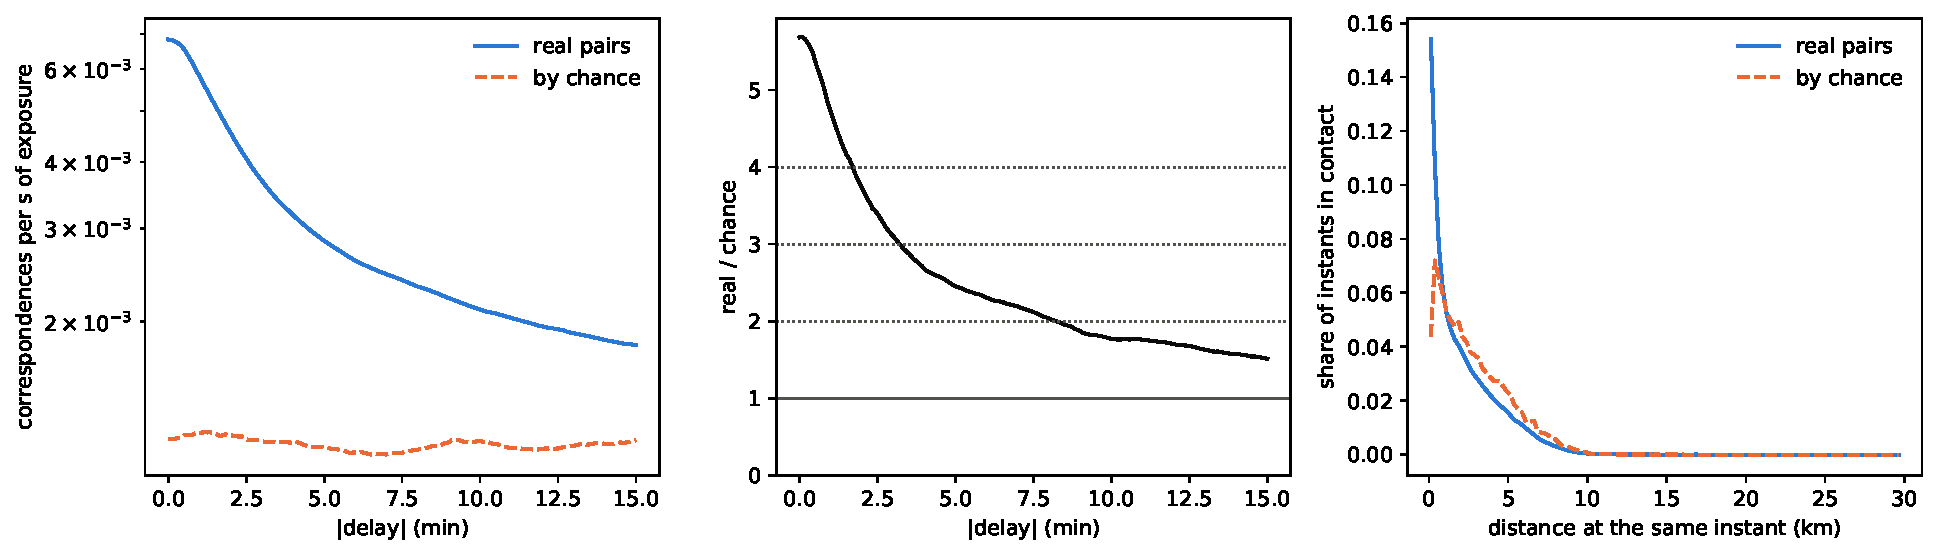
\includegraphics[width=\textwidth]{figures/assessment_delays.pdf}
\caption{The delay profile on 300 dates with a 15~min window. Left: correspondences per
second of exposure at each delay, real and by chance. Middle: their ratio $R(l)$ of
Eq.~\eqref{eq:profile}, with the levels 4, 3 and 2. Right: the distance between the two
pilots at the same instant when one is on the path of the other.}
\label{fig:delays}
\end{figure}

Chance is flat in the delay, as it should: a shifted copy has no preferred delay. The real
pairs peak at a few seconds, where they have 5.6 times the correspondences of chance, and
decay: $R$ falls below 4 at 105~s, below 3 at 195~s and below 2 at 500~s, and is still 1.5 at
15~min (Figure~\ref{fig:delays}). The excess has two parts. The fast one, within 2--3~min, is
pilots flying together. The slow one, which has not ended at 15~min, is pilots who use the
same thermals at about the same time without following each other, a synchrony that the
shifts of the surrogates remove. A rule such as ``the delay that holds 95\% of the excess''
would pick 13~min, because it counts the slow tail; that is why we read the ratio instead.

\subsection{The delay inside the contacts}\label{sec:ell}

The delay profile counts correspondences; this view looks at the contacts themselves. Every
pair interval has a delay. At each instant $t$ of $i$ in the interval with $m_{ij}(t)=1$ and
neither pilot in search, $l^*(t)$ is the delay of the closest correspondence that passes
(smallest horizontal distance); the delay of the interval is the median of $l^*(t)$, positive
when $j$ follows $i$. Its absolute value was computed for every pair interval of the run with
$\delta=5$~min, whose window is wide enough to show where the delays fall: 965\,770
intervals, of which 169\,517 have all their instants in search and no delay.

\begin{table}[h]
\centering
\small
\begin{tabular}{@{}l r c c c@{}}
\toprule
Duration of the interval & intervals & median $|$delay$|$ & within 2 min & at the edge \\
\midrule
under 10 min & 436\,575 & 210 s & 32\% & 29\% \\
10--30 min & 246\,587 & 160 s & 39\% & 12\% \\
30--90 min & 102\,357 & 80 s & 64\% & 2.1\% \\
90 min or more & 10\,734 & 25 s & 90\% & 6 intervals \\
\bottomrule
\end{tabular}
\caption{The delay of the pair intervals by their duration ($\delta=5$~min, whole archive). At
the edge: $|$delay$|\ge285$~s, the last 15~s of the window.}
\label{tab:ell}
\end{table}

\begin{figure}[h]
\centering
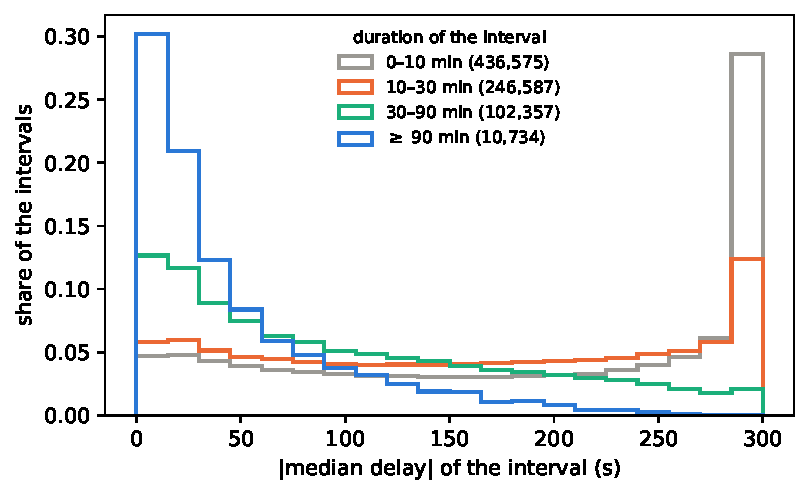
\includegraphics[width=0.62\textwidth]{figures/assessment_ell.pdf}
\caption{Distribution of the $|$delay$|$ of the pair intervals, by their duration
($\delta=5$~min, whole archive).}
\label{fig:ell}
\end{figure}

The longer the contact, the shorter the delay (Table~\ref{tab:ell}, Figure~\ref{fig:ell}). A
pair that only shares route and weather matches at any delay of the window, and its closest
correspondence is often at the largest ones: short intervals pile up at the edge, 29\% of
those under 10~min. The contacts of at least 90~min, all above $\tau^*$ of this run
(89.5~min), have a median delay of 25~s; 90\% of them lie within 2~min and only 6 of 10\,734
at the edge. Long contacts are pilots a few tens of seconds apart on the same path, which is
what $\delta=2$~min keeps (Section~\ref{sec:delta-choice}).

\subsection{Distance at the same instant}\label{sec:separation}

In analogy with the delay profile, the distance between the two pilots at the same instant was
counted at every grid instant when both fly after departure, for all the real pairs and for the
surrogates, on the dates of Figure~\ref{fig:delays} that have surrogates (210 of 300,
58\,901~h of real exposure). Unlike the right panel of Figure~\ref{fig:delays}, no
correspondence is required: every instant of every pair counts.

\begin{figure}[h]
\centering
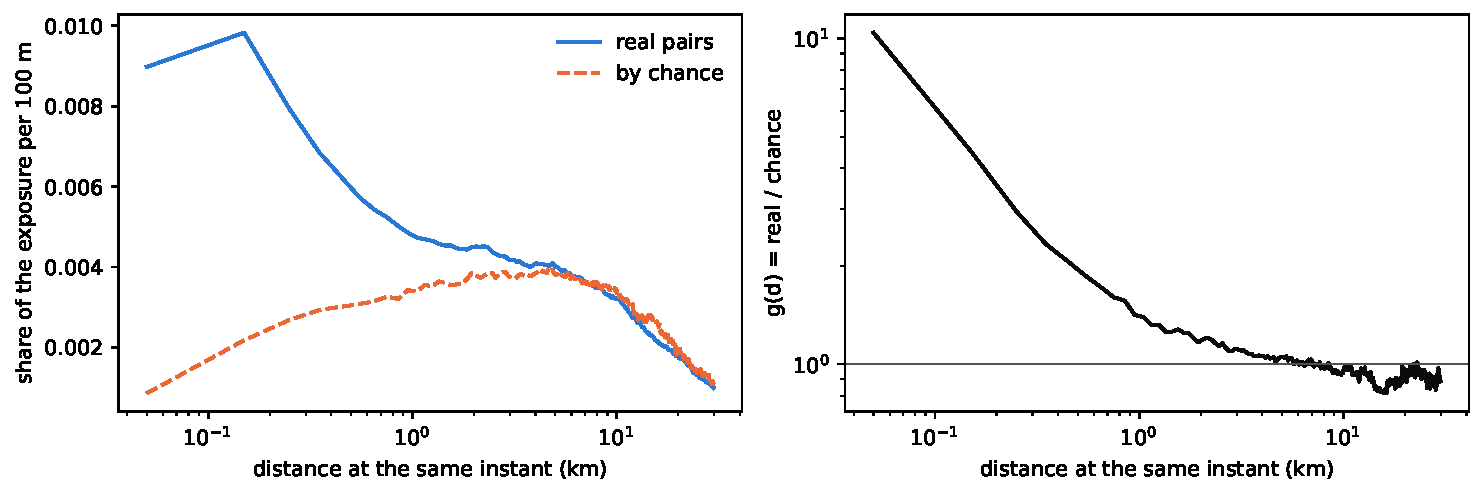
\includegraphics[width=\textwidth]{figures/assessment_separation.pdf}
\caption{Distance between the two pilots at the same instant, over all the time both fly, on
210 dates. Left: share of the exposure in each 100~m bin, real pairs and chance. Right: their
ratio $g(d)$.}
\label{fig:separation}
\end{figure}

Real pairs are much closer than chance at short distance and have no edge
(Figure~\ref{fig:separation}): $g(d)=10.4$ within 100~m, below 2 from 500~m, below 1.5 from
900~m, below 1.1 from 2.7~km and below 1 from 5.7~km. Real pairs spend 6.6\% of their time
together within 1~km of each other, against 2.8\% by chance. Beyond 6~km $g$ falls slightly
below 1, because both distributions sum to one.

The excess reaches several kilometres, beyond the visual range of 1.5~km taken in the companion
note. Since the surrogates also change the hour, this excess may hold the weather of the hour as
well as sight, so it bounds neither the visual range nor the range of following.

\section{The tolerances}\label{sec:tolerances}

\subsection{Profiles against chance}

In analogy with the delay profile, with $\delta=2$~min and the null model of the chosen run, at
every instant $t$ of pilot $i$ on the 210 dates of Figure~\ref{fig:separation}:
\begin{itemize}[leftmargin=1.2em]
\item the smallest horizontal distance between $i$ at $t$ and $j$ at $t+l$, $|l|\le\delta$,
  over the delays with $|\Delta z|<\varepsilon_z$ and headings that pass (left of
  Figure~\ref{fig:tolerances});
\item the smallest height difference over the delays with horizontal distance
  $<\varepsilon_h$ and headings that pass (middle);
\item the gaps between consecutive instants of contact of a pair (right).
\end{itemize}

\begin{figure}[h]
\centering
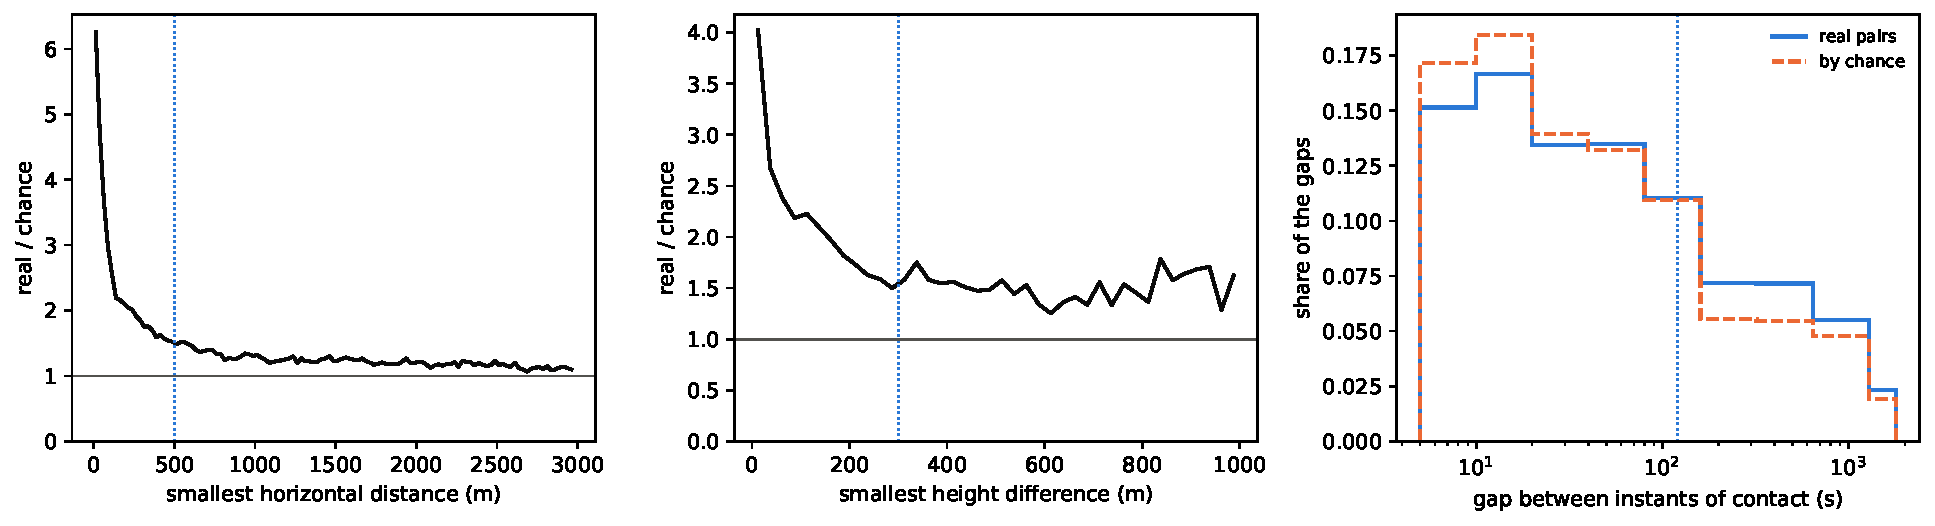
\includegraphics[width=\textwidth]{figures/assessment_tolerances.pdf}
\caption{The tolerance profiles on 210 dates. Left and middle: real pairs over chance, per
second of exposure, by the smallest horizontal distance and the smallest height difference to
the path of the other pilot within $\delta$; dotted, the values in use. Right: the lengths of
the gaps between instants of contact, as a share of all gaps (the 8\% of real and 9\% of chance
gaps longer than 30~min are not drawn); dotted, $g$.}
\label{fig:tolerances}
\end{figure}

None of the three has an edge (Figure~\ref{fig:tolerances}). The horizontal ratio is 6.3 within
25~m, below 2 from 250~m, below 1.5 from 500~m, and still 1.13 between 2.5 and 3~km. The
vertical ratio is 4.0 within 25~m and below 2 from 150~m; from 275~m on it stays near 1.5
(1.51 on average up to 1~km), the excess that the horizontal condition alone gives. Both values
in use sit where real pairs are about 1.5 times chance.

Real pairs have 1.46 times the gaps of chance per hour, because they have more contact, but the
lengths of the gaps are the same: the shares of each class differ by at most 2 points. The
gaps come from how pilots fly in and out of each other's path, the same in real and in chance
contacts, so the data do not single out $g$.

\subsection{One parameter at a time}\label{sec:plateau}

The companion note asks for a plateau: values of the tolerances around which the result does
not change. We changed one parameter at a time on 300 random dates, recalibrating $\tau^*$
each time, with $\delta=5$~min (Table~\ref{tab:plateau}). $\theta_{\max}$ changes nothing:
contacts in glide are few. The others move the fraction of flight time in a group, $f_G$, by
up to a factor three, mostly through $\tau^*$: there is no plateau, in agreement with the
profiles. On 300 dates $\tau^*$ is noisy (126~min with the starting values against 89.5 on
the whole archive, and six settings stop at the same surrogate interval); a conclusive check
needs the whole archive for each setting, about one hour each. It was not repeated with
$\delta=2$~min.

\begin{table}[h]
\centering
\small
\begin{tabular}{@{}l c c c c@{}}
\toprule
Setting ($\delta=5$ min unless stated) & $\tau^*$ (min) & $f_G$ & episodes & flights in a group \\
\midrule
starting values & 126.1 & 0.034 & 98 & 210 \\
$\varepsilon_h=250$ m & 75.1 & 0.058 & 253 & 537 \\
$\varepsilon_h=1000$ m & 126.8 & 0.065 & 162 & 372 \\
$\varepsilon_z=150$ m & 126.1 & 0.020 & 61 & 125 \\
$\varepsilon_z=600$ m & 126.1 & 0.044 & 122 & 268 \\
$\delta=2$ min & 42.6 & 0.106 & 600 & 1\,170 \\
$\delta=10$ min & 128.4 & 0.062 & 153 & 365 \\
$\theta_{\max}=30^\circ$ & 126.1 & 0.034 & 97 & 208 \\
$\theta_{\max}=90^\circ$ & 126.1 & 0.034 & 98 & 210 \\
$g=60$ s & 75.8 & 0.087 & 332 & 732 \\
$g=300$ s & 126.1 & 0.055 & 141 & 318 \\
\bottomrule
\end{tabular}
\caption{One parameter at a time on 300 random dates (7\,051 flights), $q=0.05$.}
\label{tab:plateau}
\end{table}

\section{The parameters set by the data}

\subsection{The delay $\delta$}\label{sec:delta-choice}

We take $\delta=2$~min: within it the real correspondences are at least 3.7 times chance
(Section~\ref{sec:delay}), and it contains nine in ten of the long contacts
(Section~\ref{sec:ell}). Shortening the delay also
shortens $\tau^*$, since fewer chance matches enter: from 89.5 to 51.9~min at $q=0.05$
(Table~\ref{tab:q}).

The delay also bounds how far apart two pilots in contact can be at the same instant: at most
$\varepsilon_h+v_{\max}\delta\approx0.5+27.8\times120/1000\approx3.8$~km. A
separation of 6~km, the largest we want to call a group, is never reached by one pair; a
group, a chain of pairs, can be wider. Even with the 15~min window, 58\% of the instants in
contact have the two pilots within 2~km and 94\% within 6~km (Figure~\ref{fig:delays},
right).

\subsection{The false discovery rate $q$}\label{sec:q}

$q$ is the share of chance contacts we accept among those we keep. A smaller $q$ keeps only
very long contacts and few groups, all of them real; a larger $q$ sees more groups, with more
chance among them. Table~\ref{tab:q} and Figure~\ref{fig:q} give the trade-off.

\begin{table}[h]
\centering
\small
\begin{tabular}{@{}l l c c c c c@{}}
\toprule
$\delta$ & $q$ & $\tau^*$ (min) & 5--95\% over dates & para in a group & hang in a group & episodes \\
\midrule
5 min & 0.05 & 89.5 & 79.5--91.5 & 8.9\% & 2.1\% & 6\,090 \\
2 min & 0.05 & 51.9 & 49.1--53.3 & 13.7\% & 3.8\% & 10\,553 \\
2 min & 0.1  & 38.1 & 37.0--41.1 & 21.7\% & 6.9\% & 17\,169 \\
2 min & 0.2  & 26.4 & 25.2--27.2 & 31.7\% & 13.9\% & 26\,504 \\
\bottomrule
\end{tabular}
\caption{$\tau^*$ and the groups it gives. Flights with a logger of at most 10~s and a
position after departure: 154\,598 paragliders and 6\,039 hang gliders.}
\label{tab:q}
\end{table}

\begin{figure}[h]
\centering
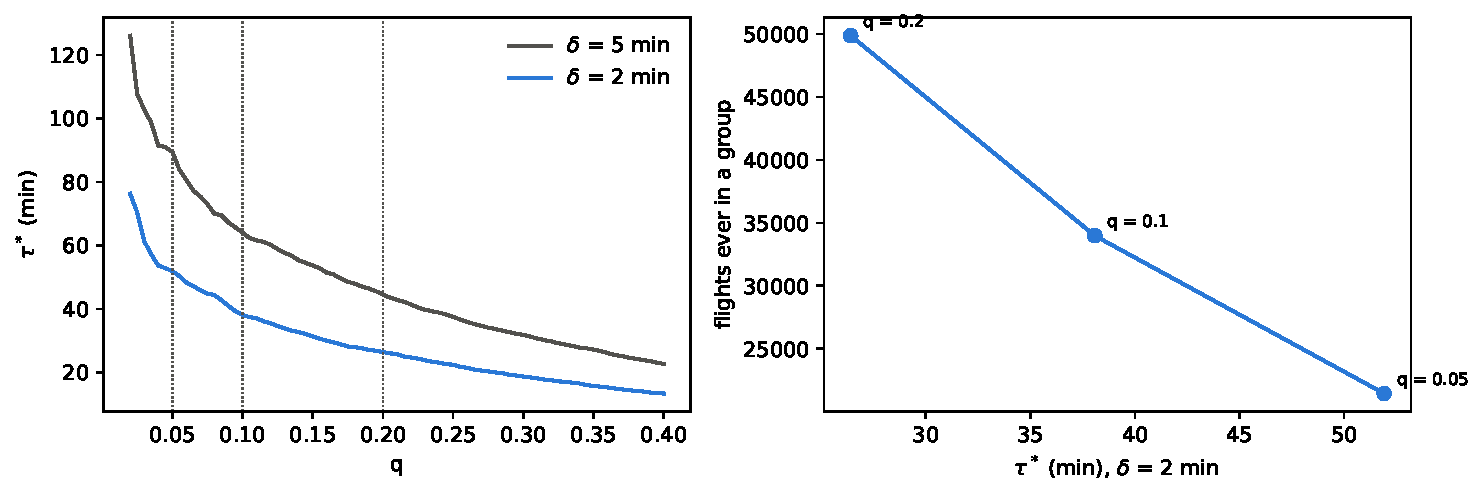
\includegraphics[width=\textwidth]{figures/assessment_q.pdf}
\caption{Left: $\tau^*$ as a function of $q$, for the two delays. Right: flights ever in a
group against $\tau^*$, for $q=0.05$, 0.1 and 0.2 with $\delta=2$~min.}
\label{fig:q}
\end{figure}

We take $q=0.1$: at most one contact in ten is chance, and $\tau^*=38.1$~min. Going to 0.2 would
lower $\tau^*$ to 26~min but would let chance make one group in five.

\section{What the groups look like}\label{sec:structure}

A configuration is a group with fixed members; it ends when a member joins or leaves. Its
duration runs from its start to its end, and its participants are its members at once. An
episode is a chain of configurations; its duration runs from the start of its first
configuration to the end of its last, and its participants are the distinct flights it holds.
The participants are counted in two ways: the share of the episodes (or configurations) of
each size, and the share of their total duration.

\begin{figure}[h]
\centering
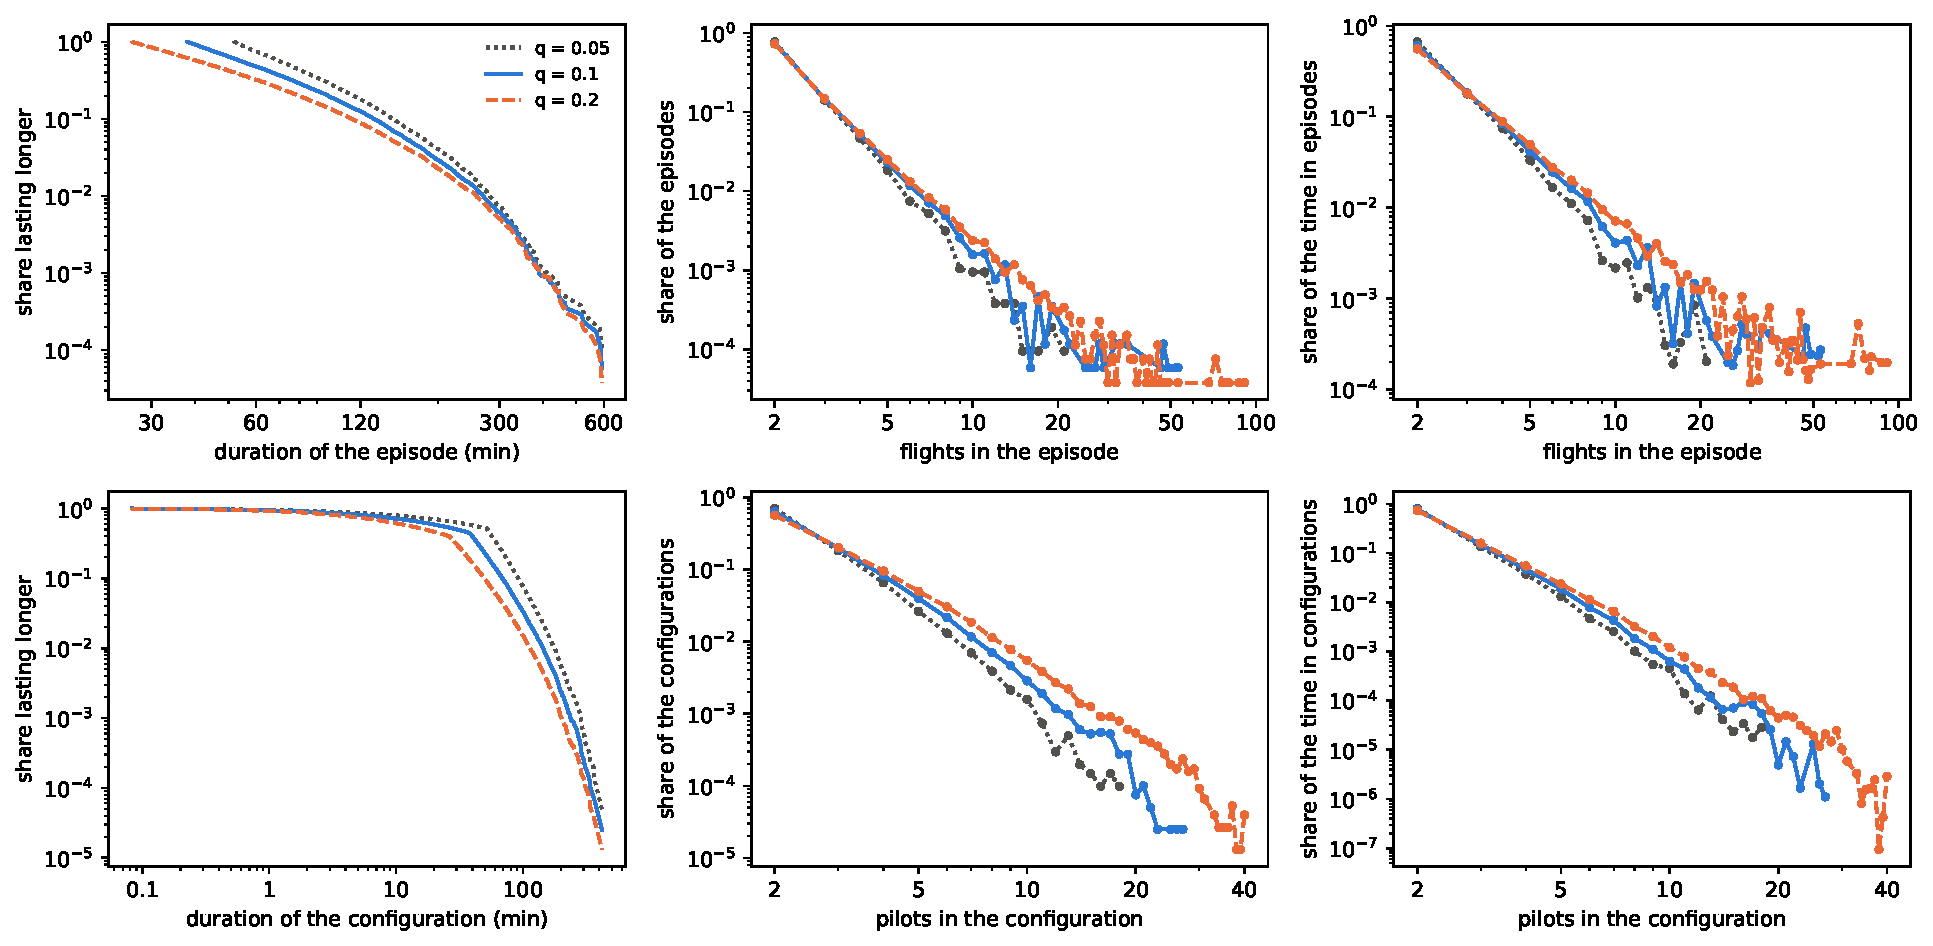
\includegraphics[width=\textwidth]{figures/assessment_structure.pdf}
\caption{Episodes (top) and configurations (bottom), $\delta=2$~min, whole archive, for three
values of $q$. Left: share lasting longer than a duration. Middle: share of each size. Right:
share of the total duration in each size.}
\label{fig:structure}
\end{figure}

\begin{table}[h]
\centering
\small
\begin{tabular}{@{}l l r r c c c c r@{}}
\toprule
& $q$ & number & median & \multicolumn{2}{c}{2 participants} & \multicolumn{2}{c}{5 or more} & largest \\
& & & duration & items & time & items & time & \\
\midrule
episodes & 0.05 & 10\,553 & 74.6 min & 77\% & 67\% & 3.9\% & 8.1\% & 21 \\
 & 0.1 & 17\,169 & 58.2 min & 74\% & 61\% & 5.7\% & 12.6\% & 53 \\
 & 0.2 & 26\,504 & 44.5 min & 73\% & 56\% & 7.0\% & 17.2\% & 91 \\
\midrule
configurations & 0.05 & 20\,275 & 52.7 min & 70\% & 81\% & 5.6\% & 2.3\% & 18 \\
 & 0.1 & 40\,051 & 30.4 min & 63\% & 77\% & 9.4\% & 3.5\% & 27 \\
 & 0.2 & 75\,953 & 17.1 min & 56\% & 74\% & 14.1\% & 5.0\% & 40 \\
\bottomrule
\end{tabular}
\caption{Episodes and configurations for three values of $q$ ($\delta=2$~min). Items: share of
the episodes or configurations of that size; time: share of their total duration.}
\label{tab:structure}
\end{table}

With the chosen values ($q=0.1$), the median episode lasts 58.2~min and three in four are pairs
(Table~\ref{tab:structure}). Episodes last at least $\tau^*$, since a contact must. Weighted by
duration the pairs weigh less, 61\% of the episode time, because larger episodes last longer:
those of five flights or more are 5.7\% of the episodes and 12.6\% of their time.

Configurations have no minimum duration: every arrival or departure of a member starts a new
one, so 10\% last less than 2.1~min, and the median is 30.4~min. Weighted by duration the pairs
weigh more, 77\% of the time against 63\% of the configurations, because large configurations
change quickly.

A larger $q$, hence a shorter $\tau^*$, gives more and shorter groups, and larger ones: the
largest episode holds 21 flights with $q=0.05$, 53 with 0.1 and 91 with 0.2. The shares of the
small sizes change little; the tail moves.

\section{Fixed settings}\label{sec:fixed}

\begin{itemize}[leftmargin=1.2em]
\item $\Delta=5$~s, the common grid: a pilot is at most 69~m from a grid position at
  100~km/h, against $\varepsilon_h=500$~m.
\item $h_{\max}=10$~s: positions are interpolated only between fixes at most 10~s apart; the
  flights of coarser loggers are left out of the statistics.
\item $R_\mathrm{dep}=3$~km: contacts around the takeoff, before the first exit from this disc,
  are not counted.
\item $v_{\max}=100$~km/h, the speed of the candidate filter: pieces of track end at every
  faster step, so the filter never misses a correspondence (checked against every pair of
  instants on synthetic days). The profiles of Section~\ref{sec:tolerances} widen the filter to
  3~km, the largest distance they count.
\item $R_s=10$~km, $r_{\min}=2\delta+\Delta$, at most 200 surrogate pairs per date: the null
  model of Section~\ref{sec:chance}.
\end{itemize}

\section{Limits}

\begin{itemize}[leftmargin=1.2em]
\item Chance is defined by the null model of Section~\ref{sec:chance}. Its shifts, about an
  hour, also remove the synchrony of pilots with the weather of the hour, so what it calls real
  includes pilots who share the same thermal at the same time without following each other:
  the ``same air'' notion of the companion note, which is not proof of interaction. $\tau^*$
  is 23~min with shifts over an hour and 53~min with shifts under 30~min
  (Section~\ref{sec:shift-classes}).
\item The profiles of Sections~\ref{sec:delay}, \ref{sec:separation} and~\ref{sec:tolerances}
  are on one sample of 300 dates.
\item The plateau of Section~\ref{sec:plateau} is on 300 dates and with the old delay.
\item The data are the cleaned tracks of the old repository (soaring, tag
  \texttt{legacy-final}); the phases needed by the heading condition exist on 1~Hz flights
  only.
\end{itemize}

\end{document}
